\documentclass[a4paper,12pt]{report}
\usepackage{CJKutf8, color, times, titlesec, geometry, indentfirst, 
            tcolorbox, smartdiagram, amssymb, graphicx, svg, pdfpages, minted, listings}
\usepackage[backend=biber,style=numeric,sorting=none]{biblatex}
\addbibresource{report.bib}
\usepackage[colorlinks=true, linkcolor=blue]{hyperref}
\usepackage[utf8]{inputenc}
\usepackage[T1]{fontenc}
\usepackage{bookmark}
\geometry{margin=2cm}
\setlength{\parindent}{2em}

\newcommand{\TODO}[1]{\textbf{<TODO: #1 will be inserted here.>}}

\definecolor{mygreen}{rgb}{0,0.6,0}
\definecolor{mygray}{rgb}{0.5,0.5,0.5}
\definecolor{mymauve}{rgb}{0.58,0,0.82}

% listing code conf.
\lstset{ 
  backgroundcolor=\color{white},   % choose the background color; you must add \usepackage{color} or \usepackage{xcolor}; should come as last argument
  basicstyle=\ttfamily\footnotesize,% the size of the fonts that are used for the code
  breakatwhitespace=false,         % sets if automatic breaks should only happen at whitespace
  breaklines=true,                 % sets automatic line breaking
  captionpos=b,                    % sets the caption-position to bottom
  commentstyle=\color{mygreen},    % comment style
  deletekeywords={...},            % if you want to delete keywords from the given language
  escapeinside={\%*}{*)},          % if you want to add LaTeX within your code
  extendedchars=true,              % lets you use non-ASCII characters; for 8-bits encodings only, does not work with UTF-8
  frame=single,	                   % adds a frame around the code
  keepspaces=true,                 % keeps spaces in text, useful for keeping indentation of code (possibly needs columns=flexible)
  keywordstyle=\color{red},        % keyword style
  morekeywords={*,...},            % if you want to add more keywords to the set
  numbers=left,                    % where to put the line-numbers; possible values are (none, left, right)
  numbersep=5pt,                   % how far the line-numbers are from the code
  numberstyle=\tiny\color{mygray}, % the style that is used for the line-numbers
  rulecolor=\color{black},         % if not set, the frame-color may be changed on line-breaks within not-black text (e.g. comments (green here))
  showspaces=false,                % show spaces everywhere adding particular underscores; it overrides 'showstringspaces'
  showstringspaces=false,          % underline spaces within strings only
  showtabs=false,                  % show tabs within strings adding particular underscores
  stepnumber=1,                    % the step between two line-numbers. If it's 1, each line will be numbered
  stringstyle=\color{mymauve},     % string literal style
  tabsize=4,	                     % sets default tabsize to ˋ spaces
  title=\lstname,                  % show the filename of files included with \lstinputlisting; also try caption instead of title
  extendedchars=true,
}

\newminted[code]{c}{frame=single,
  framesep=2mm,
  baselinestretch=1,
  fontsize=\footnotesize,
  breaklines,
  breakafter=d,
  linenos
}

\usemintedstyle{vs}

\NewDocumentCommand{\samplec}{oom}{%
  \IfNoValueTF{#1}%
  {%
    \inputminted[frame=single, framesep=2mm, baselinestretch=1, fontsize=\footnotesize, breaklines, breakafter=d, linenos]{c}{#3}%
  }%
  {%
    \IfNoValueTF{#2}%
    {%
      \inputminted[frame=single, framesep=2mm, baselinestretch=1, fontsize=\footnotesize, breaklines, breakafter=d, firstline=#1, linenos]{c}{#3}%
    }%
    {%
      \inputminted[frame=single, framesep=2mm, baselinestretch=1, fontsize=\footnotesize, breaklines, breakafter=d, firstline=#1, lastline=#2, linenos]{c}{#3}%
    }%
  }%
}

\newminted[codebash]{bash}{frame=single,
  framesep=2mm,
  baselinestretch=1.2,
  breaklines,
  breakafter=d,
  linenos
}

\newmintinline[sh]{bash}{}
\newmintinline[cpp]{c}{}


\title{{
\LARGE 健康資訊交換系統中之容器安全\\
\Large The Container Security in Healthcare Data Exchange System
\newline
\newline
\newline
\newline
\large
國立中山大學資訊工程學系\\
Department of Computer Science and Engineering\\
National Sun-Yet-San University, Taiwan \\
110 學年度大學部專題製作競賽 \\
Bachelor's degree graduation project in 2021\\
}}

\author{
Author: Chih-Hsuan Yang (B073040047)\\
Advisor: Chun-I Fan
}

\linespread{1.5}
\begin{document}
\begin{CJK*}{UTF8}{bkai}
  \maketitle
  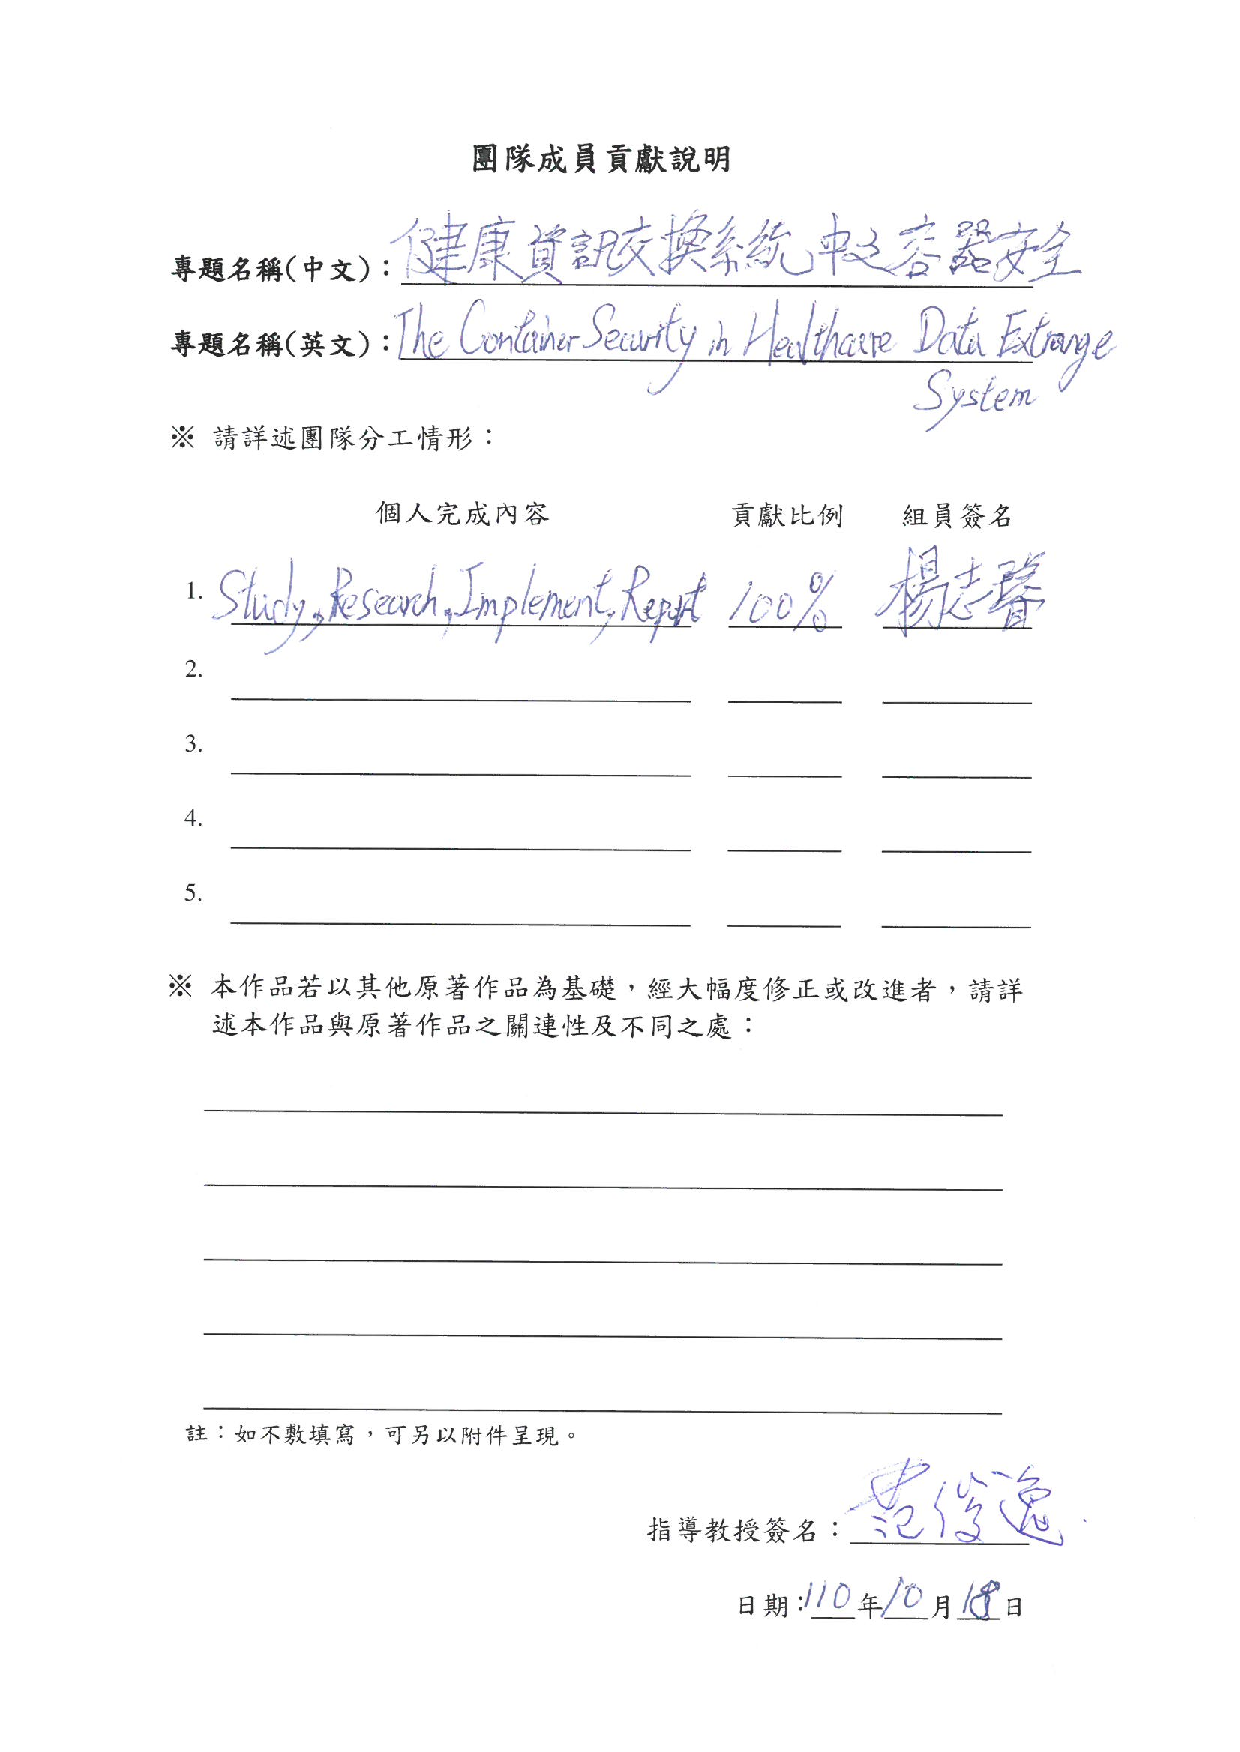
\includepdf{contribute.pdf}
  \begin{abstract}
    This research proposes
    a mechanism, forces the system to call a specific policy in the container, which is deployed in
    runtime. This policy is designed for the FHIR healthcare data exchanging in standard's container, which
    could guarantee the FHIR server to have only supported behavior and to take almost zero overhead.
    Recently, many companies use containers to run their microservices since containers could
    make more efficient use of their hardware resources as well as the newest healthcare data exchange
    standard FHIR (Fast Healthcare Interoperability Resources)
    %\footnote{{\href{https://www.hl7.org/fhir/}{https://www.hl7.org/fhir/}}}
    has been implemented
    in a container by IBM, Microsoft, and Firebase. The deployment of FHIR in a container is a trend
    in the digital world \cite{8473370}.
    Containers are isolated processes %\footnote{\url{https://github.com/google/gvisor}}
    instead of sandboxes \cite{10.5555/1267569.1267570}. Therefore, this proposed scheme could reduce the
    risk of attacks in healthcare data exchange system without performance overhead.
\end{abstract}


  {
    \linespread{1}\selectfont
    \tableofcontents
  }
  \chapter{Introduction}

\section{Container and Linux Kernel}

The container is a secondary product of the operating system in the past 20 years.
The FreeBSD develops `Jails' in 1999, and the Solaris develops `Zones' in 2004.
Linux also took this idea into the Linux kernel, which is named cgroups (2007),
the capabilities (2003), and seccomp (2005). However, why the Linux breaks this
technology into many parts? This is because they had discussed:
"Why Should a System Administrator Upgrade?" in 2001
\footnote{Version 2.4 of the LINUX KERNEL--Why Should a System Administrator Upgrade?
    \url{https://www.informit.com/articles/article.aspx?p=20667}}.
The Linux kernel almost entered the development path of "upgrade for demand" like
Microsoft Windows, and deviated from the original path of "providing a mechanism
but not a strategy" of the original Linux kernel.

While Linux were spreading in various server or distributed system, the
Linux community got more pull requests to solved the scalability and virtualization
issues \cite{267148}. However, they avoided confusion caused by multiple meanings of
the term "container" in the Linux kernel context. In kernel version 2.6.24 (2007)
\footnote{Notes from a container: \url{https://lwn.net/Articles/256389/}},
control groups functionality was merged into the mainline,
which is designed for an administrator (or administrative daemon) to organize processes
into hierarchies of containers; each hierarchy is managed by a subsystem. Moreover, the
cgroups was rewrote into cgroups-v2 in Linux kernel 4.5 (2015)
\footnote{Control Group v2: \url{https://www.kernel.org/doc/Documentation/cgroup-v2.txt}}.

The first and most complete implementation of the Linux container manager was LXC
(Linux Containers). It was implemented in 2008 using cgroups and namespaces,
and it runs on a single Linux kernel without requiring any patches. LXC provides
a new view and imagination of virtualized services without any hypervisor. In 2016,
Docker replaced LXC with "libcontainer", which was written in the Go programming language.
Docker combined features in a new, more attractive way and made Linux containers popular.

The secondary product of the operating system, containers, offering many advantages:
they enable you to "build once, run anywhere." Docker does this by bundling
applications with all their dependencies into one package and isolating applications
from the rest of the machine on which they're running. Therefore, this research
is based on docker container to propose a scheme of healthcare data exchange system's
security.

\section{FHIR}
FHIR is a standard for healthcare data exchange. The FHIR standard will be used in
Taiwan in the near future. FHIR will be used to provide PHR (Personal Healthcare Records)
in Taiwan. Therefore, we choose the most popular standard "FHIR" for the target of
the healthcare data exchange system.

\subsection{RESTful API and Data Structure}
REST (Representational State Transfer) is a stateless reliable web API, which is based
on HTTP methods to access resources or data via URL parameters and the use of JSON or
XML format to transmit queries. Because the RESTful is stateless, the client should
keep their information (i.e. cookies) by themself.

FHIR has features: RESTful and data structure, make our research and benchmarks more accurate
and reliable.
Statelessness is a developer-friendly feature, the developer and the tester would not
to design a complex state machine on the server-side or generating test files. And the FHIR
takes RESTful as standard. Moreover, FHIR standard declared the `StructureDefinition'
\footnote{FHIR Resource Structure Definition: \url{http://www.hl7.org/fhir/structuredefinition.html}}.
These structure definitions are used to describe both the content defined in the FHIR
specification itself - Resources, data types, the underlying infrastructural types, and
also are used to describe how these structures are used in implementations.

\subsection{Why IBM FHIR server}
There are many applications using IBM's FHIR server as the base component of the EHR
(Electronic Health Records) system to communicate with the other various databases.
Take it for example that the NextCloud's EHR service, Taipei Veterans General Hospital,
and AWS Cloud are using the FHIR server in a container for subroutine service.
NextCloud is an open-source and self-hosted productivity platform for users.
Many people caring about their privacy issues distrust the FAAMG (Facebook,
Amazon, Apple, Microsoft, Google), so they are using NextCloud to keep their privacy
on their own. Therefore, they are eager to have a secure EHR system for their
PHR
\footnote{\href{https://www.youtube.com/watch?v=AAP4N3KyLmM}{Richard Stallman talks about IoT}}.

The benefits of providing IBM FHIR container security in our study are providing
secure protection testing, methods, and performance evaluation for FHIR services provided by
well-known international company (IBM). This research will provide an important reference for
commercial projects for the health information exchange system practiced by medical
institutions in Taiwan.

% \section{Data and Privacy}
% Medical privacy is keeping patient records secure and confidential. In the field of software 
% engineering, each person's biological information is just a piece of data. But for living people, 
% bioinformatics is a basic human right to their human dignity.
  \chapter{Related Works}
  \chapter{Preliminary}

\section{Container's Components}
\subsection{Namespaces}
\subsection{Cgroups}
\subsection{Seccomp}

\section{Programs in Execution}
\subsection{The task\_struct in Kernel}
\subsection{Capabilities}

\section{User Mode Linux}
\subsection{Sandbox Security}
\subsection{gVisor}

\section{The (e)BPF}

  \chapter{Proposed scheme}

\section{Workflow}
\subsection{Scan Base Image}
\subsection{Signing}
\subsection{Check Image and Policy}
\subsection{Enforce Policy}

\section{Rolling Updates}
  \chapter{Analysis and Benchmark}

We profile an image of containers via cgroup and namespace
and use the seccomp mechanism to force the policy in the kernel.
We will analyze how we protect our system when hackers landing
into the container, and we profile the concurrent costs of this
mechanism.

\section{Analysis}
Our defense level is at the kernel level, but the virtual machine's
defense level is at the instruction level. Because we do not impose any
restrictions on the CPU instruction set, nor isolate the host operatin system.
Although defense level at the instruction set seems to to be more efficiency,
the virtual machine's protection consumes more time. We will show that in \ref{conc}.

In the health and medical information exchange system, the health and
medical information we protect is specialized and fixed. For example,
we do not have any attack of parsing some format string
\footnote{\url{https://owasp.org/www-community/attacks/Format_string_attack}},
which is a exploit of bypassing the ASLR \footnote{\url{https://lwn.net/Articles/569635/}}.

So we can remove some redundant system call support has reached to
limit the possibility of hacker exploitation. In order to protect
the user's data from being attacked or leaked in the information exchange system.

\subsection{Attacking Surface}
We discuessed the five stage of malware in \ref{Five_stage_of_malware}. We analyzed
three possible attack scenarios for hackers in this subsection.

\subsubsection{Administrator account leakage}
There are many situations where administrator accounts are accidentally
leaked, such as: social engineering attacks, side-channel attacks,
or account IDs and passwords known through other ways.
In 2020, 20 million household registration information in Taiwan is
suspected to be sold on the dark web\footnote{\url{https://www.ithome.com.tw/news/137955}}.

We can prevent such attacks in advance by setting up a system call filter
in seccomp. When a hacker logs into the system as a system administrator
and executes a foreign malicious program, the malicious program will call
the system out of schedule to perform malicious actions.
Even though we normally give the system administrator the highest privileges
to perform arbitrary tasks, we can analyze the behavior of the container
at build time and block unexpected behavior.

\subsubsection{Zero-day or One-day Vulnerability}
Assuming that the hacker does not have system administration privileges,
but exploits the vulnerability of the health information exchange system
(IBM/FHIR server) to conduct malicious attacks, we can also use the same
behavioral filter to filter the attack.
For example the log4j attack (CVE-2021-44228), which is a vulnerability
been published while we researching this container security issue.
Before our research, this vulnerability existed in IBM/FHIR container server
\footnote{\url{https://github.com/IBM/FHIR/issues/3156}}.
When user turns the "export to parquet" feature on, which would
brings in much of Apache Spark which leads to enable the vulnerable log4j.

But unfortunately, we have to admit that the defenses we propose cannot
withstand this log4j attack. The IBM/FHIR server itself can enable such a mechanism,
so actions using log4j are invoked at build time. We would admit these
behaviors as normal behavior in system call filter level.

\subsubsection{Breaking protection rings}

\begin{figure}
    \centering
    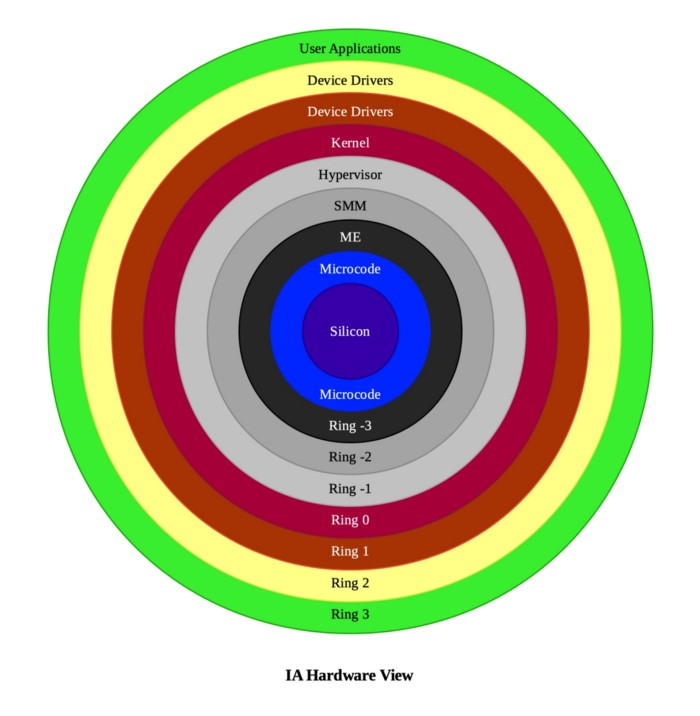
\includegraphics[width=.5\textwidth]{src/ring.jpeg}
    \caption{Intel Architecture Hardware View}
    \label{ring}
\end{figure}

Within the architecture of a computer system, a protection ring
\footnote{\url{https://www.eff.org/deeplinks/2017/05/intels-management-engine-security-hazard-and-users-need-way-disable-it}}
\footnote{\url{https://medium.com/swlh/negative-rings-in-intel-architecture-the-security-threats-youve-probably-never-heard-of-d725a4b6f831}}
, which is shown in figure \ref{ring}, is one of two or more
hierarchical levels or layers of privilege. Which was proposed by the Multics 
operating system \cite{6234805}.

Containers can theoretically have more secure ring protection in the
protection ring than in the host environment. Because the permitsions
of a container could have at most as many permissions as the host environment.
Therefore a container could break the protection ring, only if the host
machine could be cracked by those attacks which is applied in the container.

In other words, when a Container can break the protection ring, we permitted
too much capability to that container. Therefore, in our proposed method, the
system call limit during the container execution period is given at build time,
which can effectively defend against attacks such as breaking protection ring.

\subsection{Time Consuming}
\textcite{KOZHIRBAYEV2017175} showed that there is basically no
statistical difference between container and host environment.
This is completely in line with our perception of container, 
which is said that containers are isolated processes.

\subsection{Statistics}
According to our experiments, the integration tests and unit
tests were executed on IBM/FHIR server 4.9.0, and the system calls,
and system events we collected are shown in the figure \ref{hist}.

The figure \ref{hist} is the FHIR server's all system calls in
BoSC\cite{1495942} and the number of called times.
\begin{figure}
    \centering
    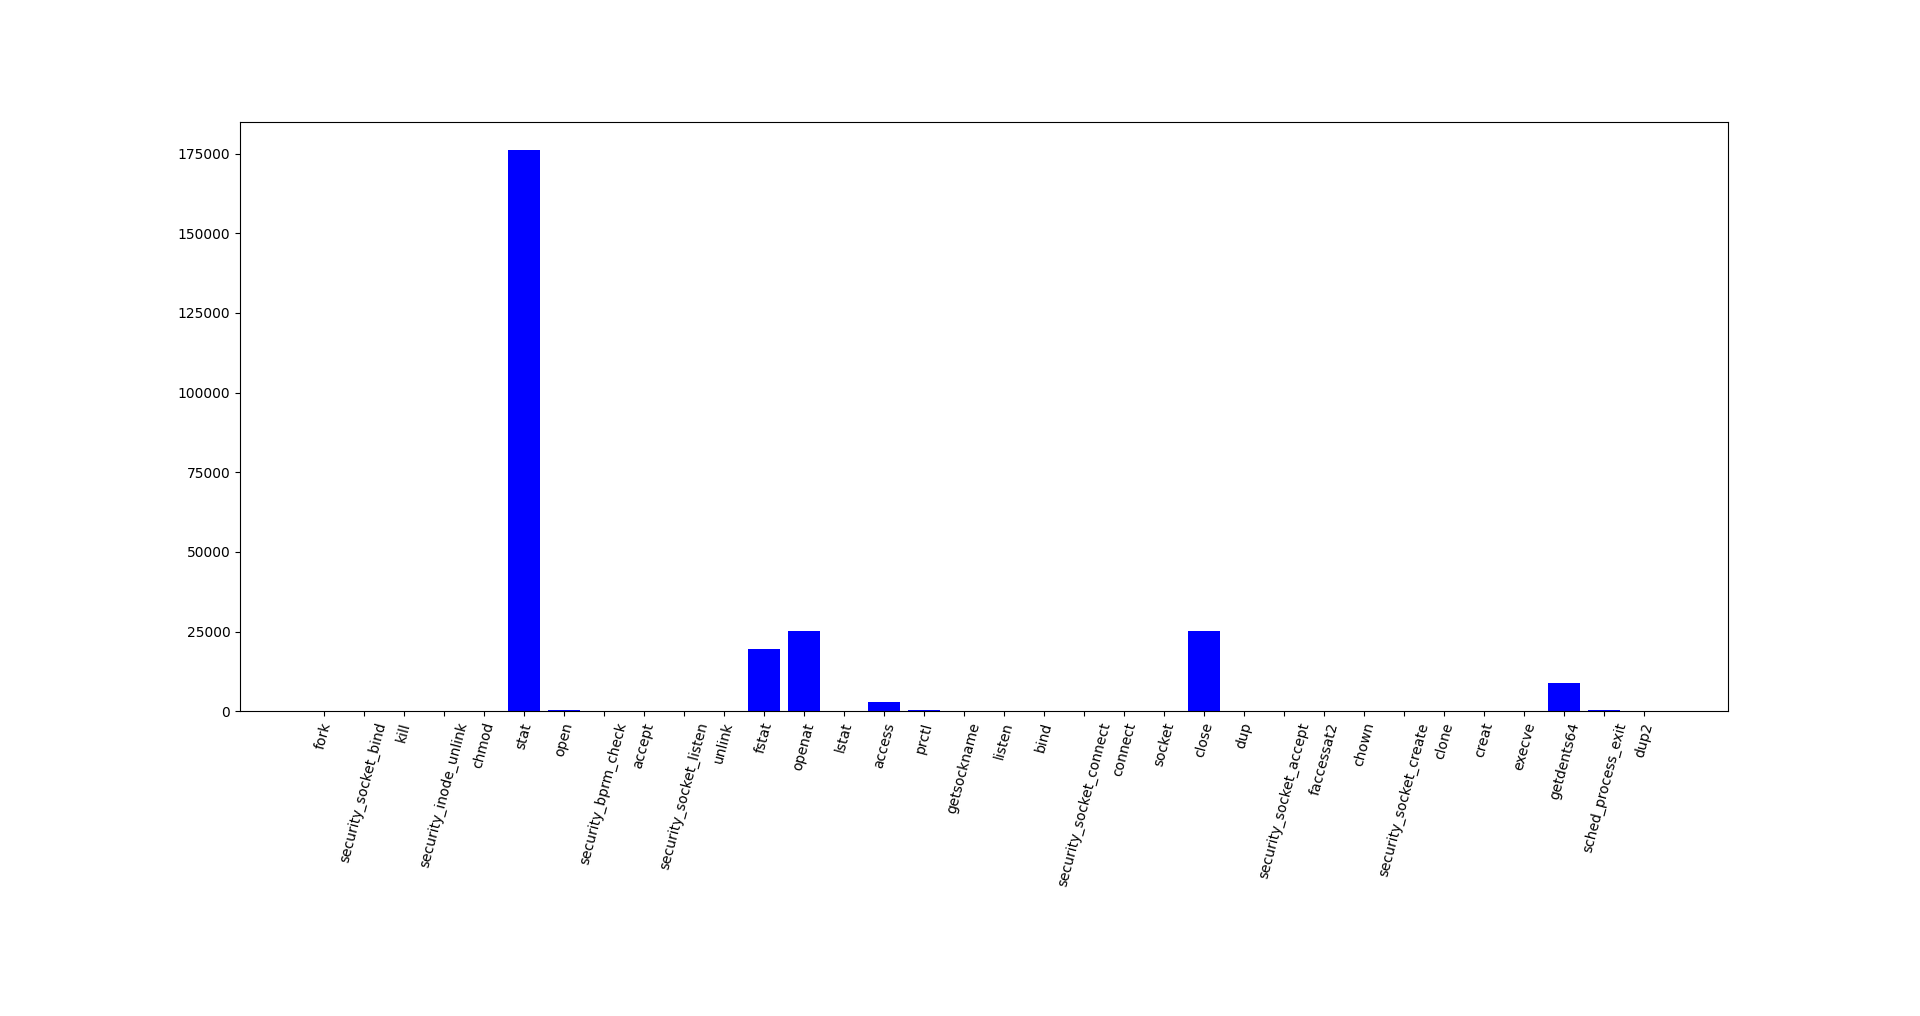
\includegraphics[width=\textwidth]{src/hist.png}
    \caption{All the system calls which the FHIR called times}
    \label{hist}
\end{figure}
Among them, we can find that the most used is the `stat' system call.


\section{Benchmark}
It is found that the discussion of container performance testing is less
focused on the requirement of parallel multiplexing
\cite{7371699,KOZHIRBAYEV2017175,7095802,234857}. And it is a more
important issue for the server's high multiplexing performance service client.

\subsection{Latency}
Figure \ref{conc} is the concurrent processes transporting time
difference in container and virtual machine.
\textcite{234857} showed that the latency of opening and closing files
are not significant difference between native and runc. But there was 12 times
faster than the gVisor with internal access. Although our IBM/FHIR server
cannot be executed in gVisor, it is the same in native and runc with no
significant difference.

\textcite{7095802} showd the relation between the throughput and the concurrency 
, both have transactions uppper bound cost in MySQL. The overhead of KVM is
much higher, above 40\% in all measured cases. We think there is a driver
buffering bottleneck in the hypervisior of KVM in ring 0.

So we compare the time lag between Ubuntu 20.04 in QEMU/KVM in Archlinux
and native Alpine container in Archlinux on concurrent requests. 
A phenomenon we found is that the latency curve of a virtual
machines seems to be different in complexity from that of a native container.

\begin{figure}
    \centering
    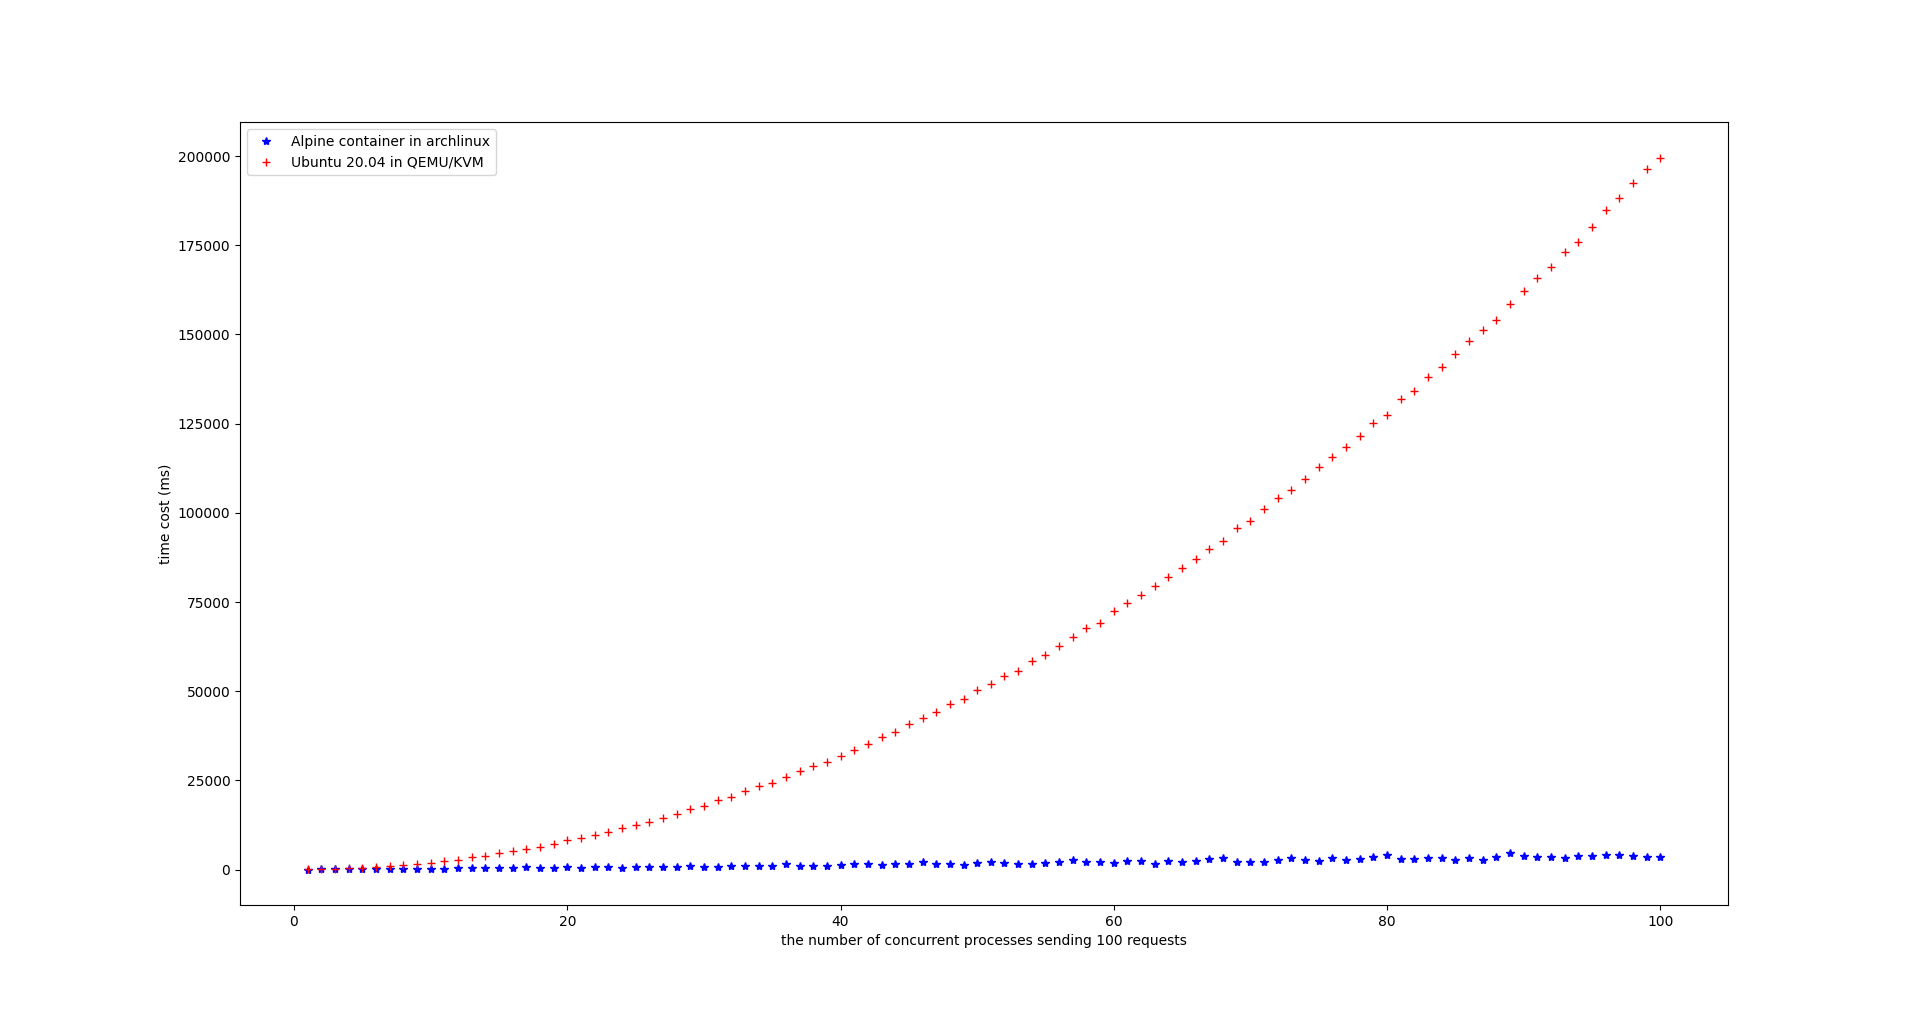
\includegraphics[width=\textwidth]{src/concurrent.png}
    \caption{Concurrent processes transporting time}
    \label{conc}
\end{figure}

  \chapter{Conclusion}

We can see the comparison results in virtual machine and container are
significantly indifferent order of time-consuming. There is no existence
of the gVisor's result because the gVisor was not able to launch the
IBM/FHIR server system, which is the target of our research.
We also expect the gVisor might run faster significantly than the virtual
machine, however, our target cannot be launched successfully in
gVisor's sandbox.

We thought there might have been some race condition bugs via JWE(JAVA Web
Engine) in gVisor. We found the IBM/FHIR server return an error code $141$
while it launching. However, we did the same configuration in Docker with
our policy and raw gVisor. Therefore, we thought the gVisor did not do
well in supporting all system calls.

And the time complexity of the virtual machine is significantly different from
the container. We propose a hypothesis of the time complexity of the virtual
machine, because there are more page fault events and limited by the
throughput of virtual machine device driver\cite{10.5555/1267569.1267570,7095802}.

\section{Better Architecture}
To better profile the IBM/FHIR server, we can start with the Hooked JVM,
which prevents unexpected objects from being generated at execution time,
such as fetching unspecified settings from JDBC. To make this method come
true, we will need to do two things: 1. JVM Hook, 2. Pre-parse the relationship
between Java bytecode and system calls.

In order to better provide the maintenance of information security for specific
applications, containerization is one of the means. In the face of more detailed
security controls, we should especially focus on more detailed patterns. The
collection system call is of course more versatile, but this is where we can
design better.

We think the problem with delay is the hypervisor's driver buffer bottleneck, but
there might be still too many variables in the middle. We need more analysis of
hypervisor and hardware communication mechanisms' formula to determine the root
causes.

\section{Future Machine Learning in Kernel}
Each FHIR request will conform to a certain format, and even when it is highly
parallel, it will have a certain pattern. We can start from the FHIR container
and put recurrent neural network or Hidden Markov Model into the kernel via ebpf.
Perhaps we will have more accurate and flexible containers to protect the health
and medical information exchange system.


  \nocite{*}
  \linespread{1}\selectfont
  \printbibliography[title=Reference]
  \addcontentsline{toc}{chapter}{Reference}

\end{CJK*}
\end{document}
